\documentclass[border=6pt]{standalone}
\usepackage{pgfplots}
\pgfplotsset{compat=1.17}
\begin{document}
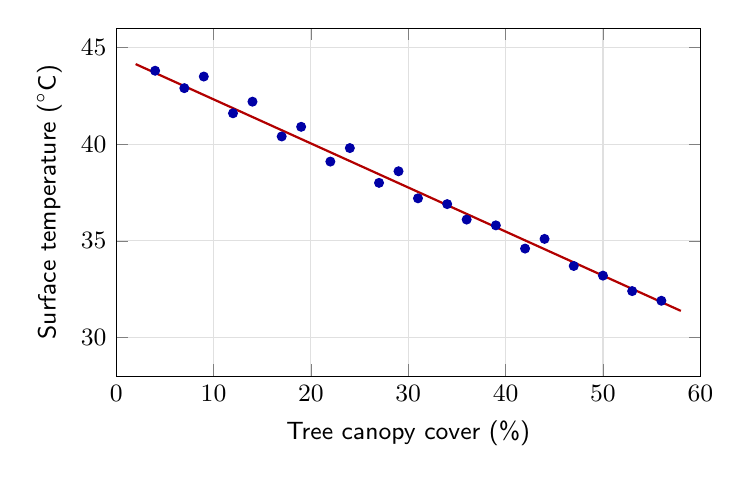
\begin{tikzpicture}
\begin{axis}[width=9cm, height=6cm, font=\sffamily\small, xlabel={Tree canopy cover (\%)}, ylabel={Surface temperature ($^\circ$C)},
  xmin=0, xmax=60, ymin=28, ymax=46, grid=major, grid style={black!12}]
  \addplot[only marks, mark=*, mark size=1.6pt, blue!65!black] coordinates {(4,43.8)(7,42.9)(9,43.5)(12,41.6)(14,42.2)(17,40.4)(19,40.9)(22,39.1)(24,39.8)(27,38.0)(29,38.6)(31,37.2)(34,36.9)(36,36.1)(39,35.8)(42,34.6)(44,35.1)(47,33.7)(50,33.2)(53,32.4)(56,31.9)};
  \addplot[red!70!black, thick, domain=2:58] {44.6 - 0.228*x};
\end{axis}
\end{tikzpicture}
\end{document}
